\chapter{Sensing in the Built Environment}
\label{chap:SensingInBuiltMain}

% Buildings consume nearly 40\% of the total energy produced in the United States and 72\% of the electricity.  Similar figures 
% have been recorded in other industrialized countries~\cite{buildings_study}.  Furthermore, studies show that they waste from
% 30-80\% of the energy they consume.  

Building management systems contain hundreds to thousands of sensors embedded in the systems that control the internal environment and
the spaces occupied by people.  There are many different kinds of sensors take a diverse set of physical measurements.
Some of them include temperature sensors in the thermostats,
valve-position sensors and actuators in the pipes, pressure sensors in the vents, temperature sensors on the vents and pipes as well, etc.
The BMS presents these through a graphical interface for building managers.  The graphical interface contains graphical sketches
of the systems and spaces in the building with icon images of the sensors in their approximate physical location represented
in the sketch.  The image sketch is generated from building schematics, so the interface is representative at the time of construction.
Building managers can quickly locate any sensor in the building through a series of clicks.

% that is giving bad readings or find the sensors that support
% a space where complaints are coming from, so that he/she could identify faulty readings through close inspection.
% The interface also allows them to visually inspect and quickly try to diagnose a problem, typically in response to occupant
% complaints.

Although BMS's have, to some degree, been an effective tool for centralized mangement of buildings, they lack the extensibility
and analytical capabilities necessary to support an ecosystem of tools for analyzing the building.  In general, software
practices in the building are non-standardized and non-systematic.
% Although BMS's have been revolutionary from a building management perspective, they lack many fundamental components for
% the kind of analysis that is needed to understand the building's operation over time.
% is performing now  
% and will perform in the future.  
% Also, building practices for software-driven building systems serve more as guideline than
% as a standard.  Naming, access, and organization of building data varies as much as buildings do.
This presents major challenges with respect to software re-use and scalability.  
In this thesis we discuss how we address these challenges through architectural design choices and analytical metholodology.  
The achitectural choices reconstruct the software layer that sits on top of existing building management systems and presents
a unified interface and standard API for analytical and control building applications.
The analytical methodology offers a general approach for verifying the construction of point names -- the naming scheme for 
sensors distributed throughout the building.  
% Both set a foundation for ongoing and future work.

The thesis is presented in the context of BMS systems and the building applications we aim to support.
% building systems and building-related applications.  
% We draw out the components in our analysis and design and discuss where it fits in the broader context of prior, computer-science related
% literature.  
In the next section, we describe the state-of-the-art practices followed by vendors of building information systems.
We describe the architectural features and design principals both implicitly and explicitly implemented into them.
We also present the pros and cons of these decisions and their implications and include a high-level description of our approach.
% Later chapters delve more deeply into the implications of our design decisions.

\section{Tightly Integrated Building Information System Architecture}

The first building information systems became commercially available in the 1970's ~\cite{gardner1987energy}.  
Historically, building management 
systems were constructed as a collection of control loops, which progressed from pneumatic to analog to digital.
These control loops largely form the foundation for the design decisions made in building information systems.  
This section gives a quick overview of the architecture, bottom-up and describes how each stage is built around
the concept of loops and supervisory control.  We then describe some of the short-comings of this architecture
and give an overview of how we address it in a system called StreamFS -- described in more details in
the remaining chapters.

\begin{figure}[t!] %htbp
\centering
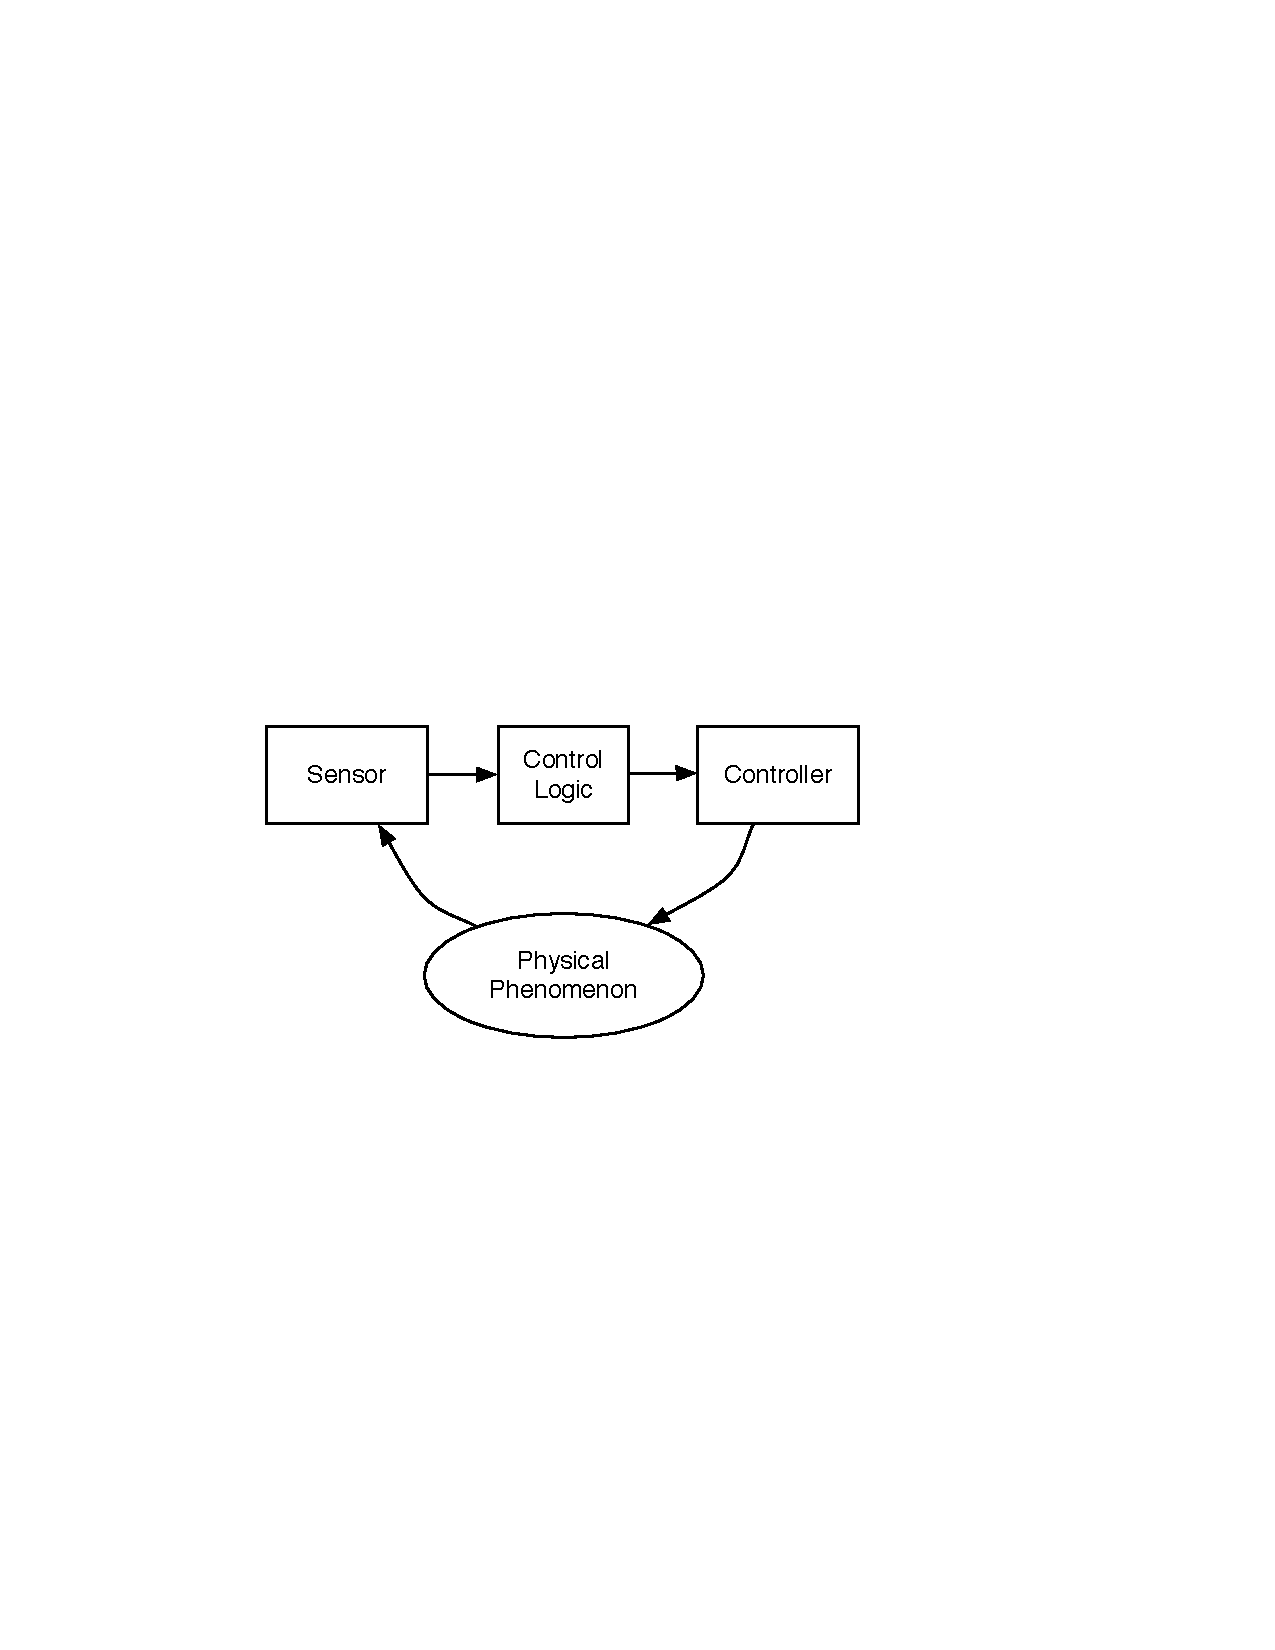
\includegraphics[width=0.50\columnwidth]{figs/control_loop}
\caption{General building control loop.}
\label{fig:control_loop}
\end{figure}

\subsection{Control Loops and The Outstation}
\label{sec:control_loops}
Each loop is defined by a control domain consisting of a sensor, an actuator, and a control mechanism.  The control mechanism
become logic based when signals from sensors moved to the digital domain.  However, the basic control principle is based
entirely on local control loops, with the implicit assumption that these loops are independent.
Figure~\ref{fig:control_loop} shows a high-level control loop.  A simple control loop in the building is one that controls
the temperature in a space.  It has a temperature sensor as the input and uses the temperature set-point parameter to 
decide when and which actuators to activate.
For temperature control, this actuation controls the the vent that lets cool air into the space.  This causes the temperature
to fall until a lower-bound is reached and the control logic re-activates the fans and heating/cooling system.

The figure also shows the basic structure inside an outstation.  An outstation is a box that contains up to several control boards, each
wired to one or more sensors and one or more actuators.  The outstation is typically close to the sensors and actuators (in the same room)
and contains all the control logic for the local plant.  Inside the control logic there is a CPU and some memory.  The memory
contains the control program and some space for sensor readings.  It is directly wired to the sensors and actuators through
a series of buses and shown in Figure~\ref{fig:control_box}.

\begin{figure}[t!] %htbp
\centering
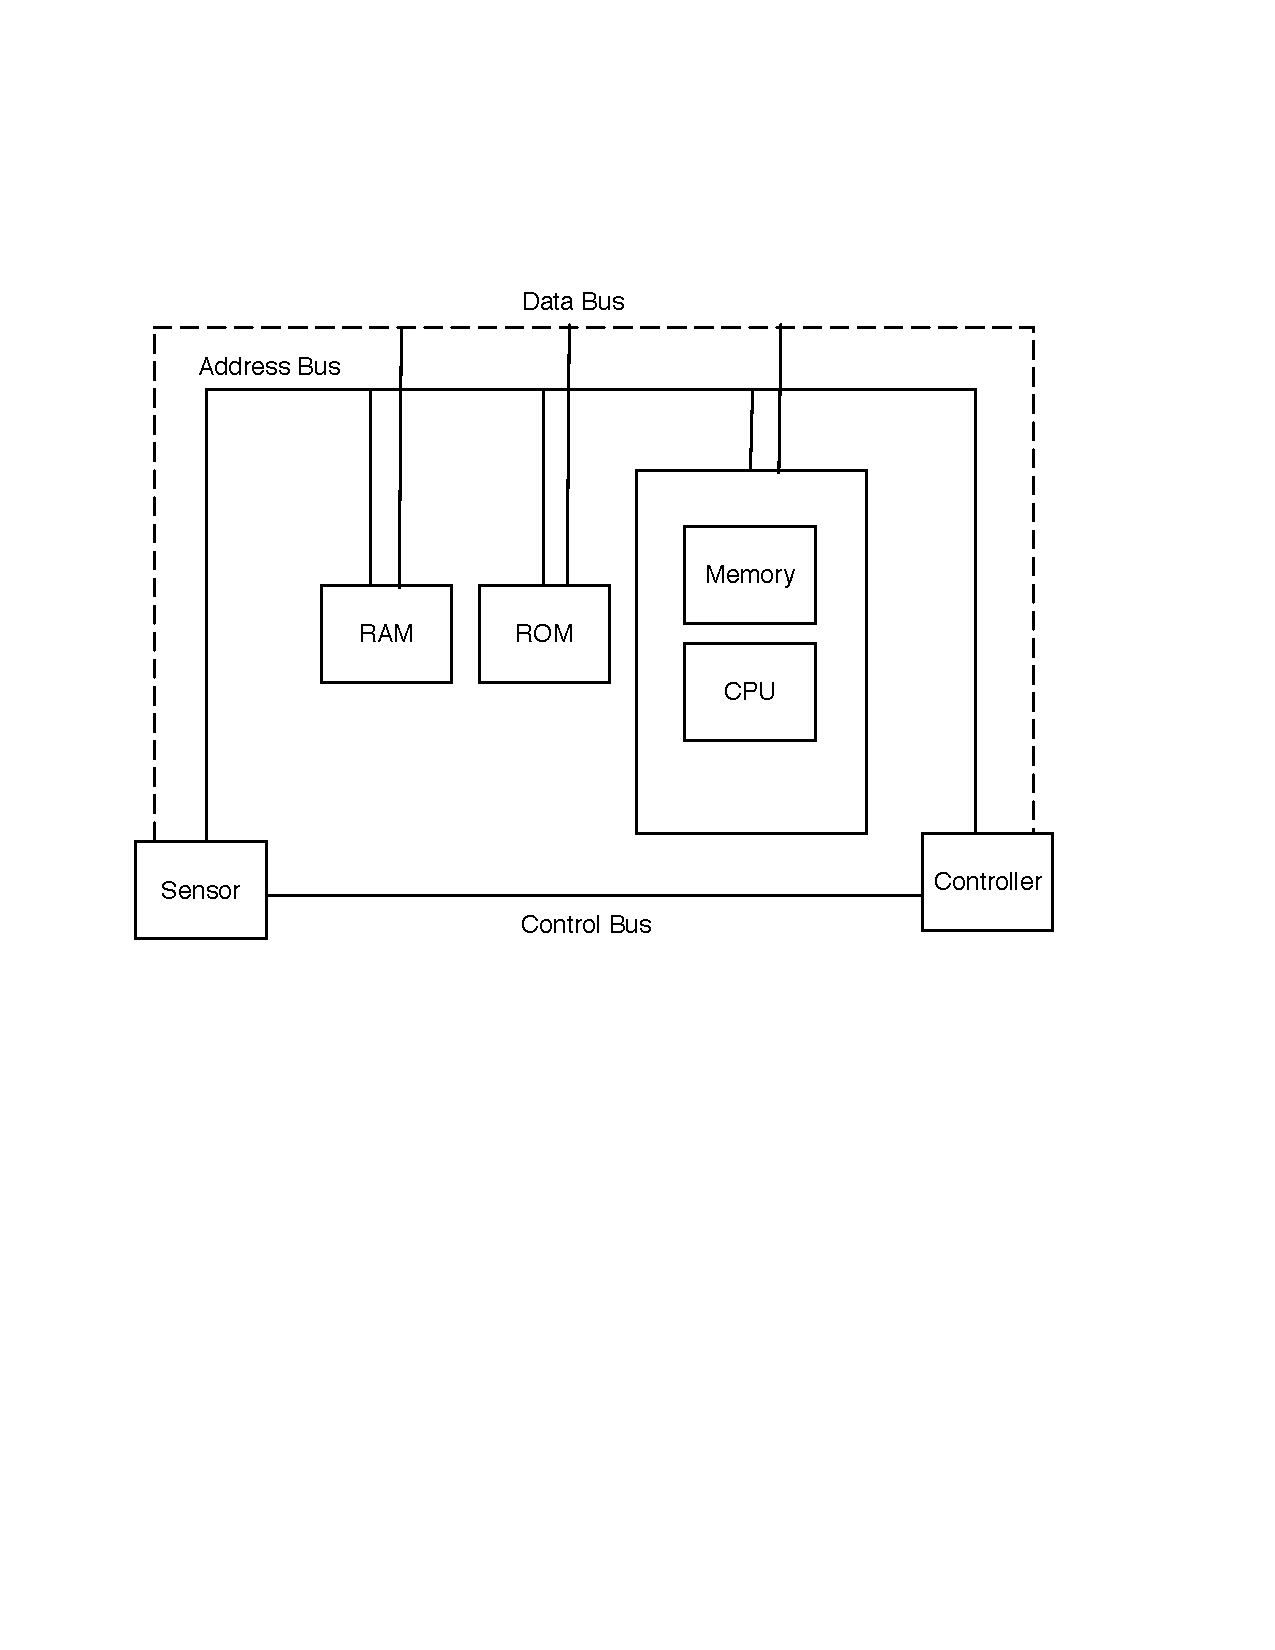
\includegraphics[width=0.50\columnwidth]{figs/control_box}
\caption{High-level control board architecture.}
\label{fig:control_box}
\end{figure}

As readings from the sensors are taken, they are placed in RAM.  The amount of RAM is limited and can get filled up, so it is important
to schedule periodic collection tasks from the central station -- the building management system (BMS).  The control logic is typically
written in ROM and can only be changed by the equipment or BMS vendor.  The input parameters are set at the BMS and they dictate the operational dynamics
of the control scheme in reaction to the input~\cite{BMS_book}.
Outstations are distributed through the building and are essentially running independent of one another.  In order to enable centralized 
monitoring and control, they are networked together and report some of the sensor readings and control-logic state to a central outstation.

\subsection{Central Outstation and Communication Protocols}
The central outstation is typically a Microsoft Windows-based PC connected to the outstation through either RS-485/modbus or Ethernet.
The user interacts with the system through a graphical interface, constructed from the schematics for the building or the schematics
for the component in the system that is being monitored.  The BMS running on the PC communicates with outstations through either a 
vendor-specific, proprietary protocol or an open one like BACNet~\cite{Bacnet} or LonTalk~\cite{LonTalk}.  Note, 
we focus on BACNet, but the similar features exist in other protocols, such as LonTalk.  

\begin{figure}[h!] %htbp
\centering
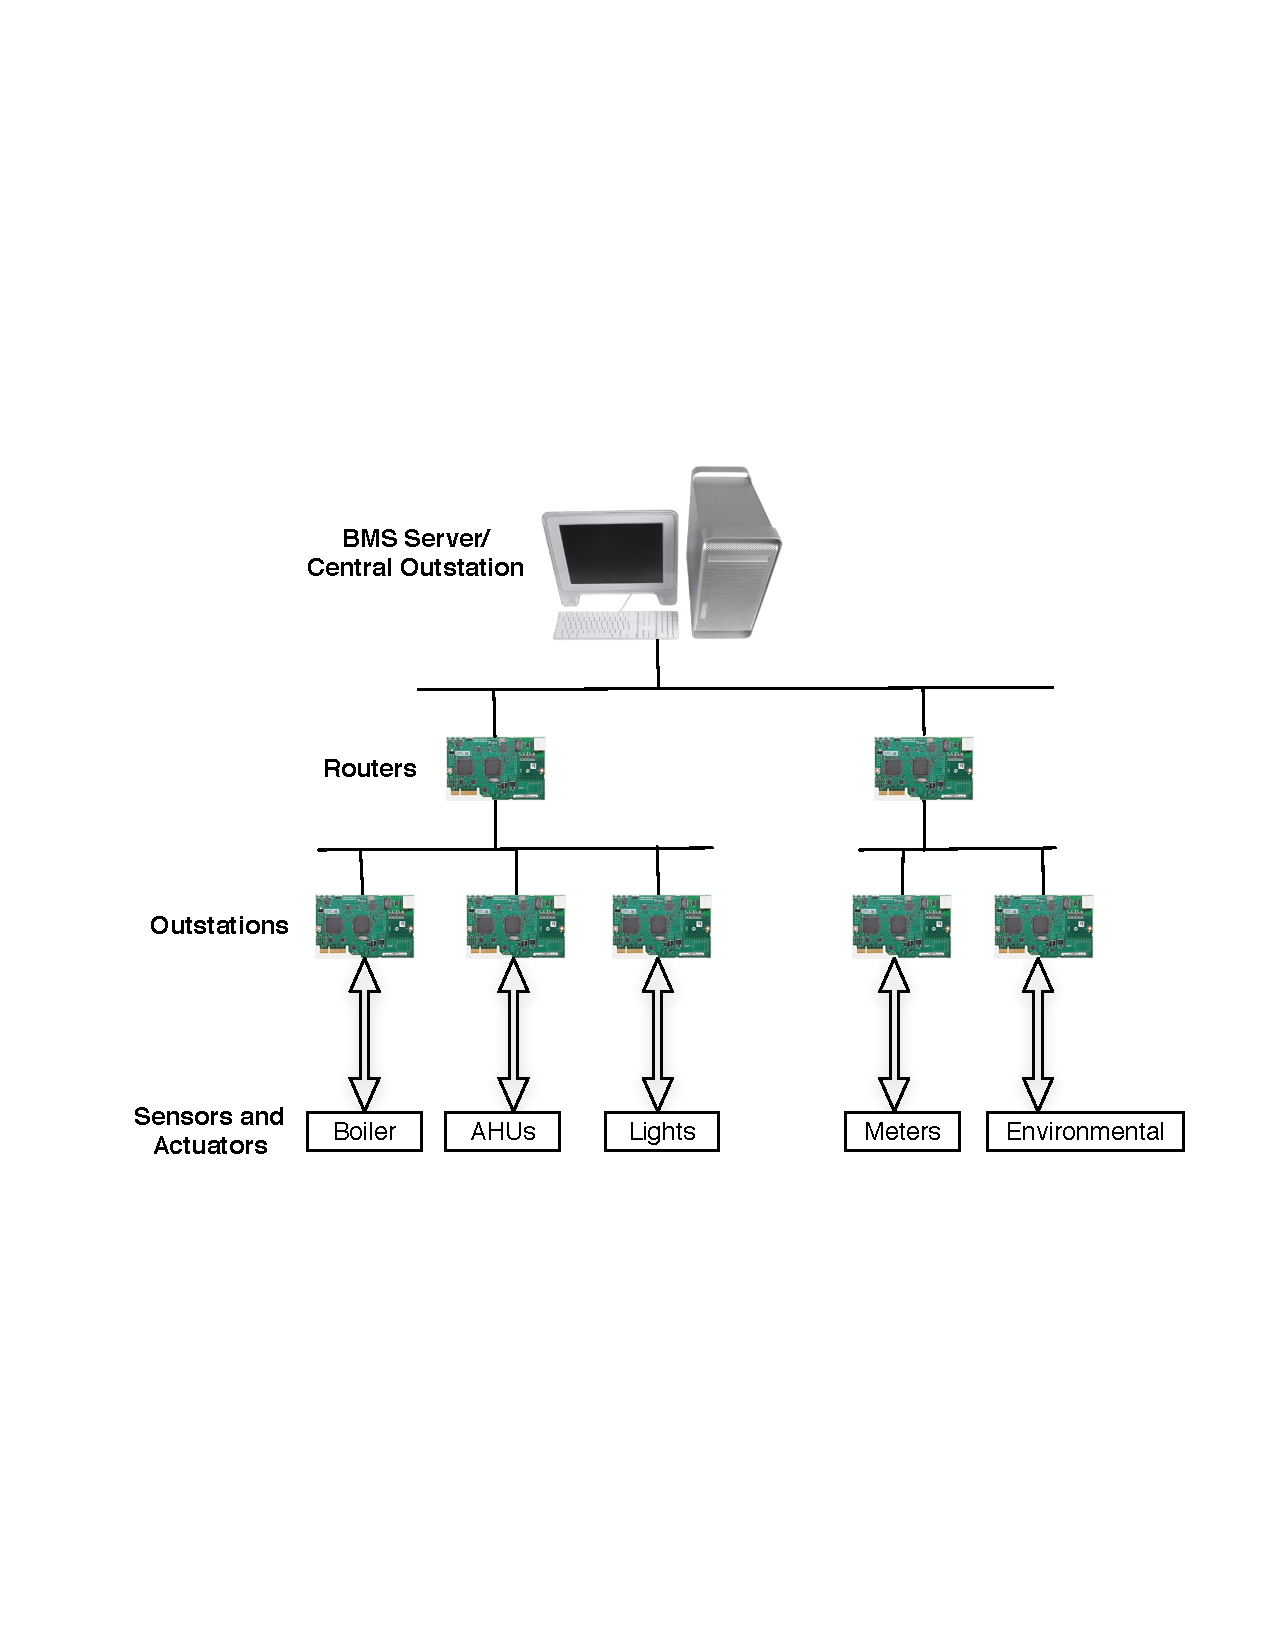
\includegraphics[width=0.50\columnwidth]{figs/BMS_network}
\caption{BMS network architecture.}
\label{fig:bms_network}
\end{figure}

Both protocols define both a wire protocol and packet structure for communicating with outstations and each other.  They also define a high-level
naming scheme for sensors in the building, called `points'.  A point can also refer to a non-physical object, like a schedule of operation.
It is common for both lights and temperature sensors to run on a daily, weekly, and seasonal schedules.  Such schedule are captured
by the \emph{schedule object} in BACNet.  
% BACNet also exposes devices as a collection of different object types.  
Each object contains a set of properties that can 
be read and/or written.  A device is identifiable through a name or address on the network, each object has a unique identifier and is one of
many types.  Examples of object types includes the following: input, output, value, analog~\cite{Bacnet}.  

These protocols also provide a mechanism for discovery .  Each [device, object name/id, property name/id] tuple forms a name.
This name is exposed by the protocol-server to the application.  All the names are set by the vendor and the are shown through the graphical interface
of the BMS.  
% constructed from the building schematics, is also designed and constructed by the vendor.  
The building manger is the primary user of the BMS,
so rather than expose the underlying protocol, he/she interacts with the building via the graphical interface.

In order to interact with the underlying sensor and actuator layer, the application must use a stub that communicates directly with the 
sensor/actuator through the BACnet stack.  External communication stubs are recognized similarly to sensors/actuators.  They are represented 
as a collection of 
objects with readable/writable properties.  An example service that is provided in BACNet is  \texttt{WhoIs} and \texttt{EventNotification}.
The former is a broadcast service that is used for discovery of other objects, the latter is used for setting alarms on the sensor data that
are reported by the BACNet enabled devices on the network in the outstation layer.  There are many other types of events that are supported 
and over 50 types of object types in the baseline protocol, which is extensible.  Device and object names that are added have no restriction
on either the number of characters (specified by the vendor) or the encoding.


\begin{figure}[t!] %htbp
\centering
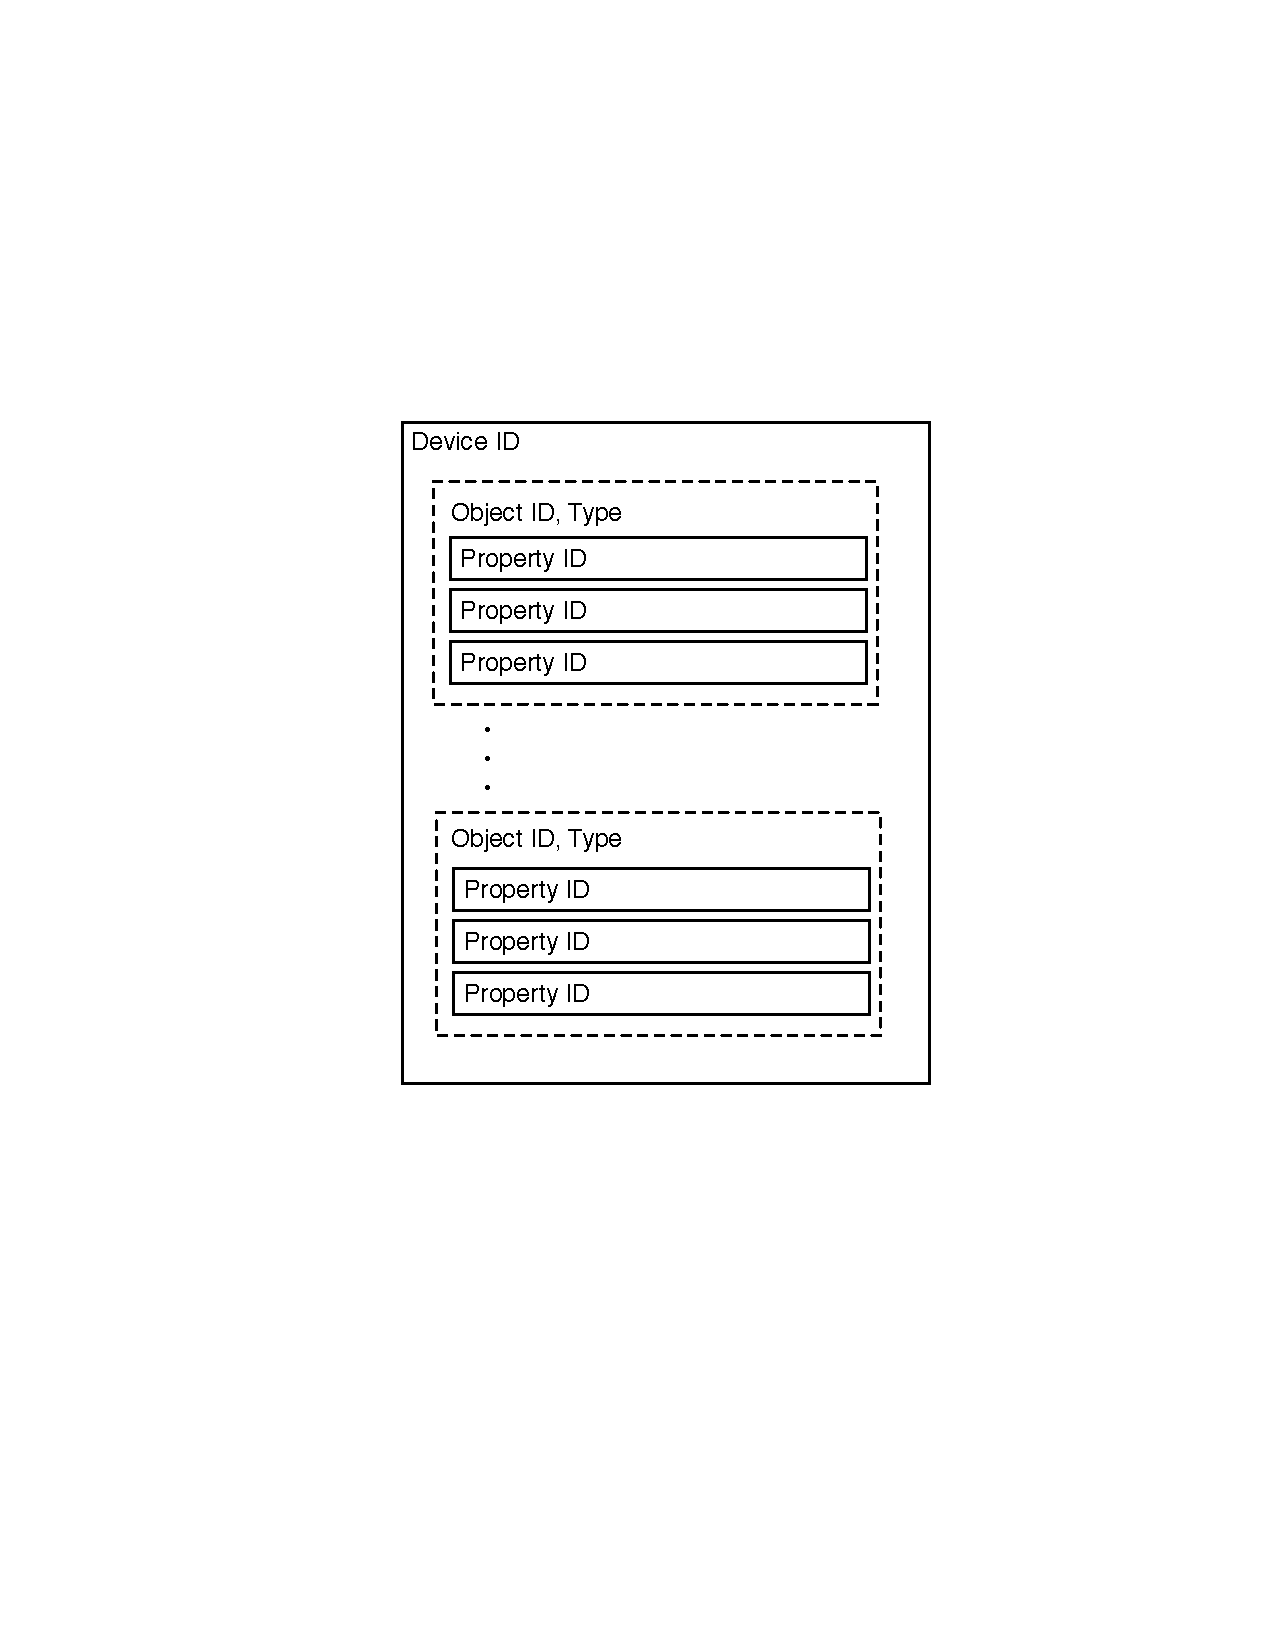
\includegraphics[width=0.25\columnwidth]{figs/bacnet_device}
\caption{BACNet device example.}
\label{fig:bacnet_device}
\end{figure}
\section{From Supervisory Control to Application Development in Buildings}
%From Supervisory Control to Application Development in Buildings

% Building information systems were built as tightly integrated silos, where the main application is the graphical user interface.
Features for interoperability were designed at two interface layers: 1) the protocol layer and 2) the presentation layer through a
data-export feature.  The protocol layer provides services for enabling devices to talk to one another through the network.  
Several features were explicitly designed around
the notion of interoperability: trending, scheduling, management services, alarms and events, direct sharing.  The graphical
interface layer is mainly focused on providing periodic reports in a comma-separated value (CSV) file, which
contains point-name information and time-value pairs of data.
% Historically, the extent of interoperability objectives has included mainly the introduction of new devices onto the network or
% the exporting of data for other software program to use for analysis and report generation.  
For these protocols, interoperability means adding new devices or exporting the data in a common format.
Building information systems themselves
were built to mainly support the in-time management and supervisory control of the building.  Analysis does not 
extend far beyond univariate plotting and individual assessment of equipment and control.  Most tuning of control parameters is 
manual.  Hard-wired control logic at the outstation is rarely updated.


Over the last few years, however, there has been in increased interest in energy management and comfort as a primary objective 
in the design of new building applications~\cite{6146507,Yu1956572,Mamidi2343582}.  Moreover, there is a broad interest in buildings
using global control schemes to optimize their performance and to interact more efficiently in response to renewable sources and its  
generation volatility~\cite{Taneja2223873,5985456,Lu2009}.  Model predictive control has introduced new ways of controling the components in the building
to make them more energy efficient~\cite{mpc}, there is an interest in performing dynamic, real-time analysis of building health
and efficiency~\cite{dynamicLeed}.  There has even been interest is improving the visibility of the state of the building to the 
occupants through various modalities, including touch-screens and mobile phones~\cite{andrew_lighting, Hsu1878444, Ortiz2422540}.  
These, and other emerging applications,
have pushed the boundaries of demand beyond what a modern building information system can provide and a re-design must be considered.
\section{BMS Architectural Shortcomings for Supporting Emergying Application Development}

\begin{figure}[t!] %htbp
\centering
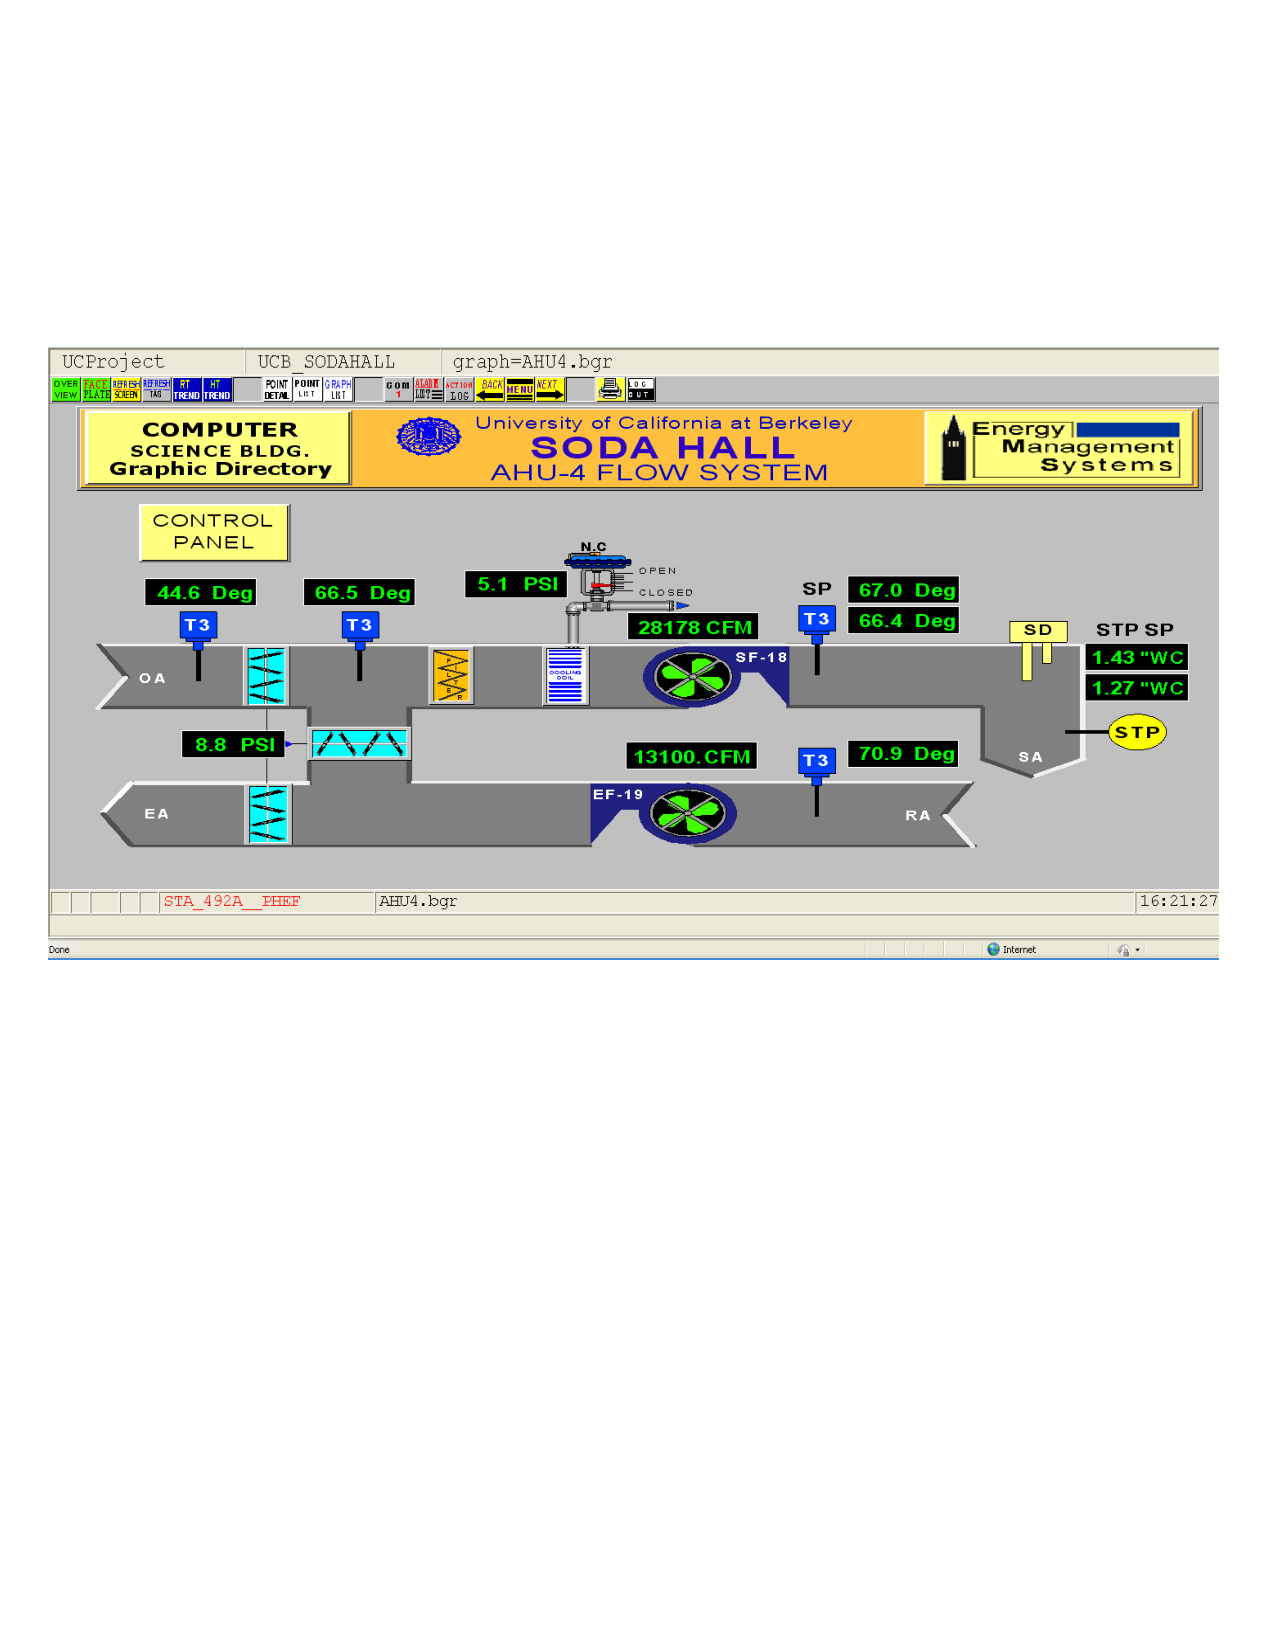
\includegraphics[width=0.75\columnwidth]{figs/soda_bms_screenshot}
\caption{Screen shot for the Soda Hall Building Management System Interface.}
\label{fig:soda_bms_screenshot}
\end{figure}

% In this section we dissect the current architecture in the context of current and future applications
% for buildings.  The first two describe how the current architecture is used to provide the intended service
% that these application provide.  The latter two are emerging applications that we would like to available
% throughout the entire building stock.  We will see, however, that these are very difficult to build at scale
% and we pose the question ``what is missing in the current architecture to enanble the system properties that help
% support these and other emerging applications?''.  Through close inspection it will hopefully become clear that
% the current architecture is fundamentally flawed; built largely to support a small set of vendor-specific
% applications and not much else.

% In this section we dissect the BMS architecture and closely examine how well it can support broad application development
% in buildings, rather than the single supervisory control function it supports today.  
We examine today's BMS architecture in the context
of 4 potential services with distinct operational requirements that need to be supported.  The first two services that 
are offered today and enabled by the BMS.  We describe how emerging requirements are driving the evolution of these
services and how BMS's are struggling to meet the new requirements due to limitations in their architectural design.
The next two are emerging services that BMS's cannot support today.  We describe which architectural components must be included
or how current components must be modified in order to support these.  We also make the broader argument that 
building systems should be built to support a much wider range of applications that we cannot currently anticipate.
We will show why this requires a fundamental re-design and propose an architectural composition for such a system.
In the rest of the thesis, we will examine an instance of our architecture and describe the challenges in realizing
the use and effectiveness of our system in real building deployments.

% while the latter are potential applications we imagine will be supported in future
% smart buildings.  Through this exercise, we build our argument for a systematic re-design of such systems and propose
% a set of necessary architectural components necessary to enable and support emerging applications.

\subsection{Monitoring and Supervisory Control}
The primary objective in the design of building information systems is for centralized monitoring and supervisory
control.  Control algorithms are left ``to the expert'' and embedded in the outstation control board.  The intended
user of the system is a building manager -- a user whose expertise is much broader than the designer of the control
algorithm that runs on a particular system component.
The manager is expected to monitor the health of building systems and quickly diagnose problems when they occur.  The tool
is mainly in place to save the building manager time; and it is very effective at doing so.  The extent to which 
the building manager is making control decisions is altering control algorithm paramter setting through
the building management interface itself.  Even these decisions typically go through the vendor, through consultation.

Figure~\ref{fig:soda_bms_screenshot} shows a screenshot of the BMS in Soda Hall at UC Berkeley.  This specific image
captures a schematic for one of the air handling units.  It shows the various sensors embedded in different locations
on the component -- on either side of the supply/exhaust fans, temperature sensors at the supply/return sides of the
air ducts and the inlet vent, measuring the outside air temperature.  Accompanying real-time readings are juxtaposed
by the sensor image.  The user can double-click on the sensor or reading to get more information about that particular 
measurement point.  For example, if you double-click on a temperature sensor, it will give you the exact name of the 
point and accompanying information about related points, such as the set-point, which effectively drives the behavior of 
the underlying system.  If an occupant makes a complaint about not getting any air from the vents, for example, the 
building manager can find the screen for the vents that serve the room the occupant is in and observe the current
pressure readings or look for value-based alerts on any of the readings, typically displayed on the same screen.
If there is a malfunctioning component or something stuck in the vent, the readings should ``look off'' to the building 
manager.

If the problem recurs often, the astute building manager may be able to characterize the fault through a series of alarms.
They can be proactive about finding and fixing the problem(s) before they occur.  Alarms can be set through interaction
with the graphical interface, in much the same way that a lookup on the measurement point occurs -- by double-clicking on 
the point in question and following instructions for setting an alarm.  In some cases, the problem may be driven 
by a faulty setting and adjustments can be made to the control parameters through the associated control points.

The scope of control is limited to specific control loops.  Recall our discussion of control loops in section~\ref{sec:control_loops}.
The building manager can, typically with the help of the vendor, decide on the best control strategy setting.  If the control
strategy cannot be met, due to flaws in the control algorithm itself, the vendor may step in and re-image the controller
at the outstation and expose the necessary parameters through the graphical interface.  These kinds of changes are rare
but do happen occassionally and can be somewhat expensive, since the cost is not typically included with the purchase
of the system.  Because of the cost, the decision is typically made after close inspection and analysis, which a BMS
enables through the data export feature.  
For example, the sense/control points in question may be placed in ``trend'' mode.  This means that readings
from those streams are stored in the local memory buffer at the outstation for some period of time.  If a report is specifically
set up at the central system, a report period is also associated with the point, allowing the saved points to be drained
from the local buffer at the outstation.  The points are then placed in a file for observation and graphing by the 
building manager.  Time-dependent inspection of the behavior of any of the control-loop related points can be examined.

Although this feature is not necessary in order to change control paramters, it is useful for observing how parameter changes
affect the behavior of the system.  The building manager can, in principal, experiment with different setting and allow
empirical observations to guide her future decisions.


\subsection{Energy Auditing and Building Modeling}
Recently there has been renewed interest in the energy consumption of buildings.  In particular, several studies~\cite{BuildingEnergyData,
MITBuildingScience} show that buildings consome a large fraction of the energy produced in the United States and that as much
as 80\% of it is wasted.  As such, there has been an emergence of several companies and services for assessning the health of
commercial buildings with respect to their energy consumption.  Organizations such as LEED~\cite{Leed} provide certification of 
buildings, specifically rating the energy efficiency of the building.

Building modeling has been part of building science for quite some time, with systems such as EnergyPlus~\cite{eplus}.
EnergyPlus and simulators like it are part of a larger ecosystem of software for modeling various aspect of the operation
of the building.  They allow the designer to construct detailed models of the building, from construction to usage.  You can
model everything from the material, location, zone-based usage (office building, bathroom, storage room), window size and its
construction, etc.  There are different types of LEED certification, but typical certification requires the submission of the detailed
model and the results of various energy-related metrics, aggregated over seasonal time intervals to attain LEED certification.

Detailed model construction can take several months and in order to ground the underlying model in empirical performance data
typically a modeler will use the data obtained from the building's BMS.  Most vendors provide a way to export the point-related 
trended data.  Complex models can be built using this information.  The file export feature in combination with the ability to 
``trend'' points provide an interface mechanism for these and other kinds of applications that need to make use of the data.

Another option is to obtain the data directly from the system through the network.  Third-party vendors provide systems that 
will join the building network of devices and eavesdrop of the readings and traffic being reported to the central server.
This is the only way to obtain truly real-time readings from the sensors on the network.
Typically BMS vendors do not like this since they may generate too much traffic and overwhelm the network because of congestion.
Although not fundamental, it is a common concern in buildings today.  Many buildings use RS-485 rather than ethernet and there is
a general, albeit unfounded, concern that the network will become overwhelmed if all the points are trended and report at the same
time.

Building modeling and real-time analysis have been separated because of these constraints.  The constraints are largely not
fundamental, but the current architecture is simply not designed to provide real-time readings for \emph{all the points, simultaneously}.
Also, it is clear, even from the fairly simple workloads generated by these analysis applications, that a history of readings
is needed.  BMS's, as currently designed, require the end-user to manage the history of the data point individually.
When BMS's were first designed, there were certainly concerns about bandwidth and storage limits.  However, today those concerns
are a non-issue.  A few hundred bytes produced on the order of a few minutes, even from several thousand sensors is simply not
that much data.


\subsection{Holistic Building Optimization}

\begin{figure}[t!] %htbp
\centering
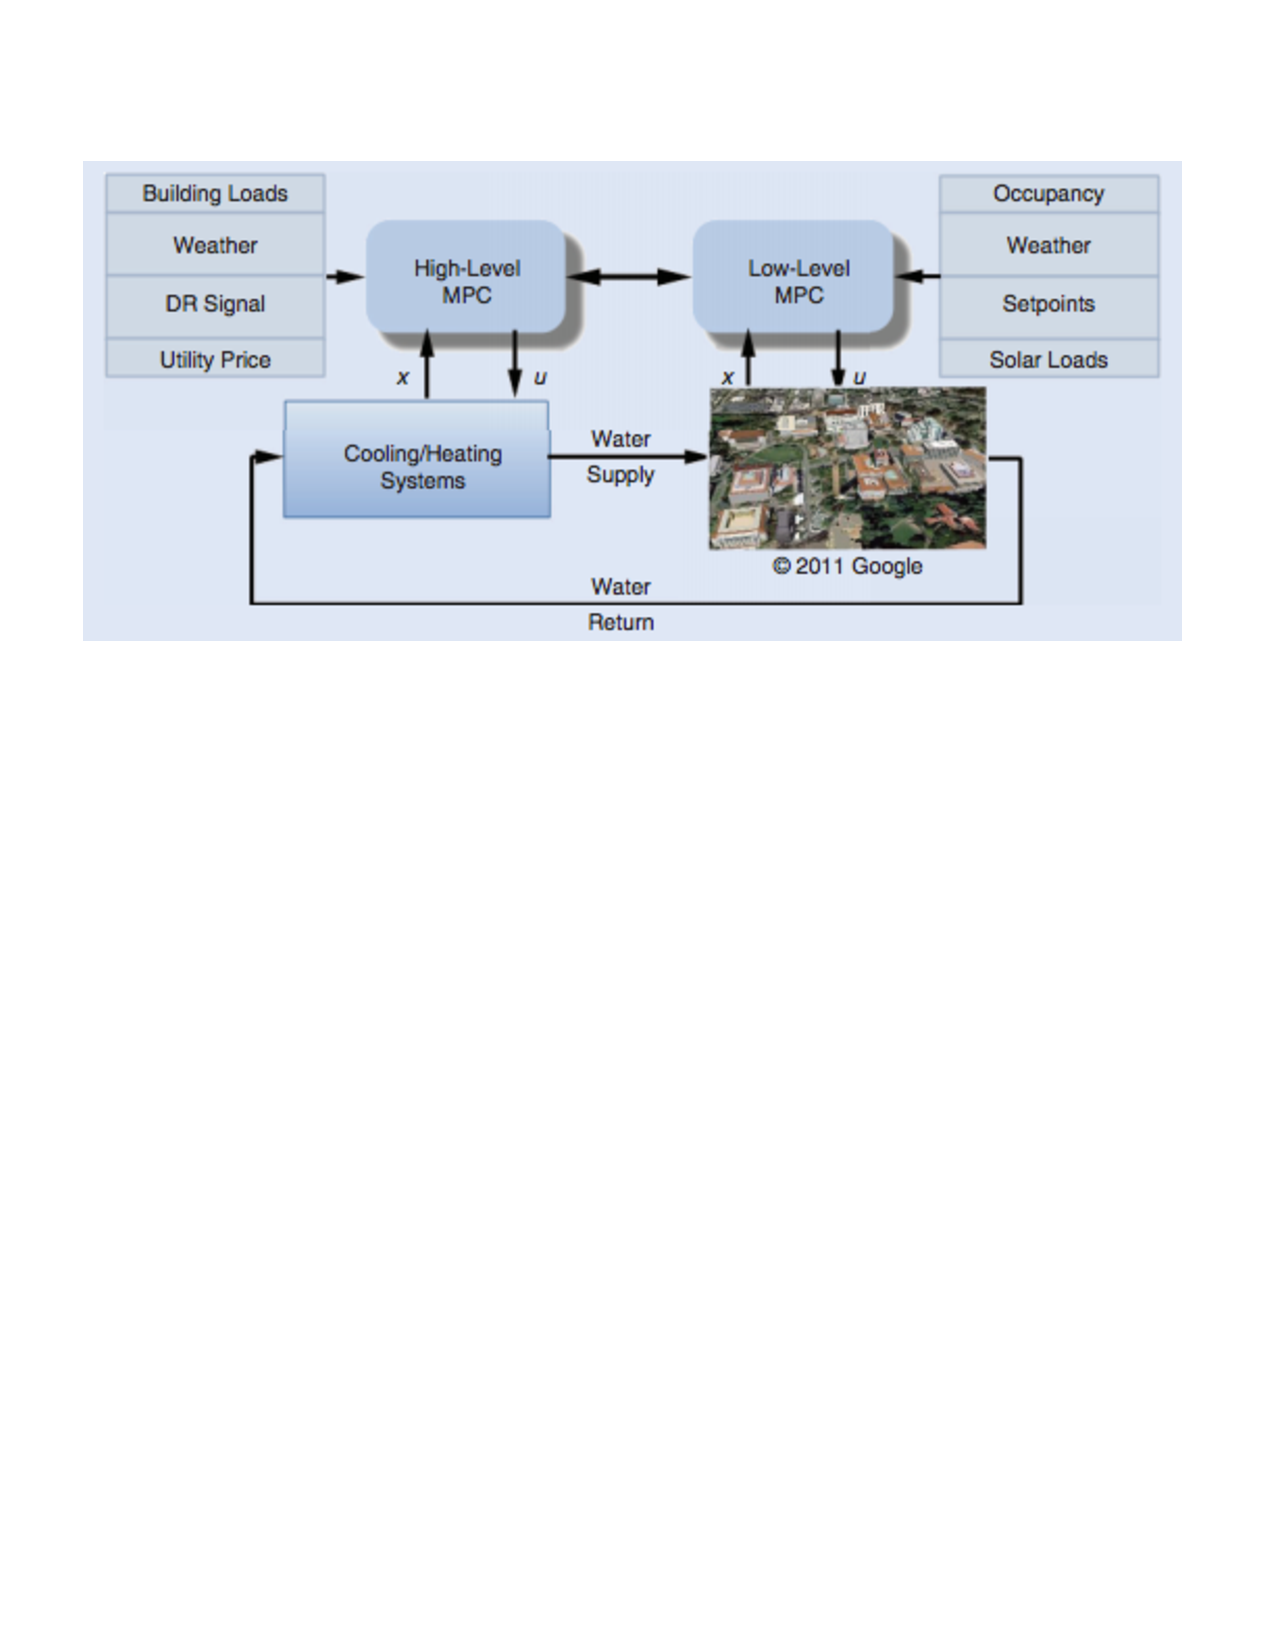
\includegraphics[width=0.75\columnwidth]{figs/mpc1}
\caption{Emerging Application: Hierachical MPC for a stock of buildings.}
\label{fig:mpc1}
\end{figure}

An emerging class of applications, is in holistic control of the building using a new technique called model-predictive control~\cite{MPC}.
Rather than rely on specific changes to control logic at the local-loop level, MPC techniques observe and learn a model
of the behavior of a components, multiple components, or the whole building, based on the historical data.  Once the model is learned, 
constraints can be specified to drive the behavior of the system to an optimal region in the tradeoff space; solving it as 
a constraint optimization problem.  Figure~\ref{fig:mpc1}, reproduced from~\cite{MPC}, shows an example of the how MPC combines 
several points in the building to control the building.  Essentially it decomposes a large optimization problem into indivial control 
decision to be made at the control-loop level.

In order to build this application, the set of necessary points must be mapped into the process.  The user, setting up the problem,
must connect the right data streams and control points to the algorithm by either manually going through the schematics or
locating the schematic representation in the BMS graphical interface.  There is no query interface and it requires that you sit
with the building manager or vendor in order to set up the trending, reporting, and enable the necessary control permisions.
The process is time consuming and \emph{does not scale}.

Although the method is very useful and has yielded excellent results, it is difficult to replicate.  The code and setup must be 
customized for each building or stock of buildings it is set up on.  This lack of generalizability and scalability is missing
in the current state of the art of building information systems.  In most cases the representation of sensor/actuator association is 
implicitly represented in a combination of the schematics, the graphical interface, and the point name.  Moreover, all
three of these change from building to building.  It is fundamentally difficult to generalize.  Buildings are treated as one-off constructions
and their associated digital information has historically followed the same principle.


\subsection{Personal Energy Viewer}
\label{sec:mobile}

\begin{figure}[h!] %htbp
\centering
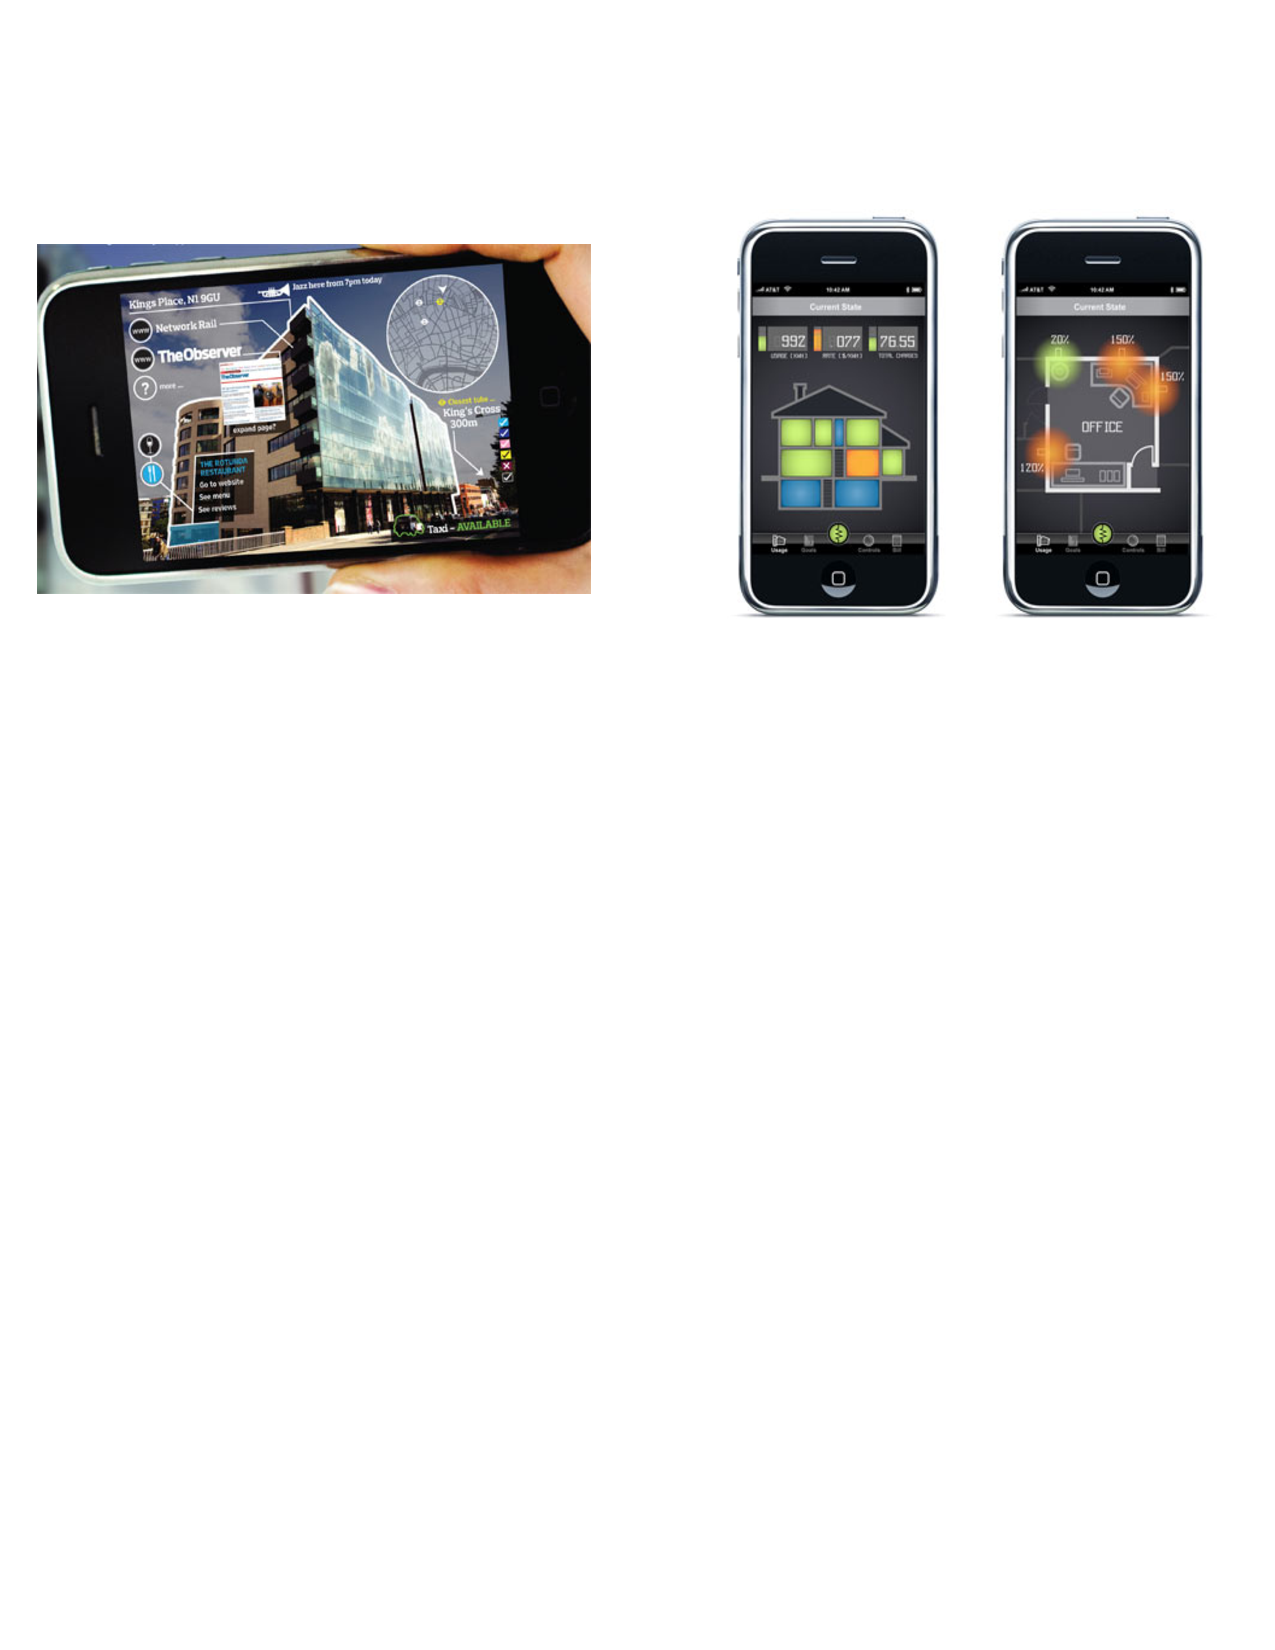
\includegraphics[width=0.75\columnwidth]{figs/mobileEnergy1}
\caption{Emerging Application: Mobile phone interfacing with the physical infrastructure.}
\label{fig:mobileEnergy1}
\end{figure}

Imagine having the ability to walk through a building and see live, detailed energy data as
you point your phone at various things and locations.  As you enter the building, you scan its tag and see
the live breakdown of energy consumption traces, including HVAC, lighting, and plug-loads.  You continue
your walk through the building as you head to your office.  When you arrive to your floor
you scan the tag for the floor and observe similar figures, only this time they are in relation to that floor
alone.  Since there are several meeting rooms on that floor, you are curious how much is consumed by 
occupants versus visitors.  You choose to view the total load curve co-plotted with the occupant
load curve, specifically for that floor.  You see that approximately half the total energy is consumed
by visitors during the day.  

Curious about what portion of total are attributed to you, you select the 
personalized attribution option and you see \emph{your} personal load curve plotted
with the total load curve -- as well as accompanying statistics, such as the percent of total over time.
As you quickly examine the data on your phone, you see that you consumed energy during hours that you were not
there.  You choose to see a more detailed breakdown.  You enter your office, scan various items that you own, and see that
your computer did not shut down properly and your light switch was set to manual.  You immediately 
correct these.

Being able to interact with your environment and get a complete energy break-down can provide a useful tool
for tracing and correcting rampant energy consumption.  In buildings, having the occupants actively participate
allows for localized, personal solutions to efficiency management and is crucial to scaling to large buildings.
However, providing this detailed level of attribution is challenging.  There's lots of data coming from various systems 
in the building, and integrating them in real time is difficult.  Furthermore, attribution is non-trivial.  
We must be able to answer to following: How much of the total consumed on this floor went to charging laptops?  How
many of those charging laptops belong to registered occupants of this floor?
For centralized systems, multiple locations are served simultaneously.  It is non-trivial to determine the exact
break-down for each location.  At the plug-load level, some plug loads move from place to place throughout the building
over the course of the day.  Tracking where they are at any given time is difficult.

Answering these queries is relatively easy once the information is available, however, collecting the information
is non-trivial, especially over time.  Historically, it has been difficult to collect plug-load information.
Various studies have used wireless power meters to accomplish just this~\cite{stephscale, lanz, aceee}.
All previous work collected the data and performed post-processing to analyze it.  We want to take the next
natural set of steps: perform processing in real-time and present the occupants with live information.

Currently, in order to enable this application, a detailed digital model of the building is necessary, data streams from the building must
be easy to query, and it should work across buildings.  Also, there needs to be a way to localize the user. 
Localization technology and information must be made available to the mobile application to provide in-situ services.
It's clear that the current information instrastructure cannot provide these.  The interface to the network does not have
a strict naming mechanism, there is not explicit representation of each building that the application could interpret, 
the sensor/actuator deployment is not dense enough and adding new sensor is cumbersome.  Furthermore, the data itself can be quite dirty.

Cheap sensors are unreliable.  They produce erroneous data and randomly stop and start at times.  Missing/errorneous data is common.
Moreoever, within building information systems provided by a single vendor, there is no time synchronization across sensors, so
aggregation, filtering, and re-sampling are common operations that must be performed on the data in order to summarize and display it.
The mobile energy viewer application not only require these but requires that they be performed in real time.







\section{Addressing BMS Shortcomings}
\label{sec:shortcomings}
% The current architecture of building systems is very tightly integrated and based on monitoring and supervisory control
% of local control loops.  
% Building systems were built as tightly integrated systems with a single application.  
The main layer of interaction between applications and BMS's is the underlying network layer and the data-export component.  
The BMS export feature decouples the protocol from the information about each sense/actuation point; time-value
pairs and the name of the point. As auditing applications emerged and energy became a prime target for reduction in buildings, 
these interface choices became insufficient.  Moreover, as the need to construct new classes of applications emerges, the architectural
pieces that are missing become more clear.  The following is a list of some of them:

\begin{enumerate}
% \item Network protocol details should remain opaque to end-user applications.
\item Narrow waist should be above the network layer. \label{nw}
\item A time-series store is necessary. \label{ts}
\item Mechanisms to distill the readings must be availble. \label{proc}
\item Real-time data forwarding should be available, especially for control applications. \label{rt}
\item Contextual relationships between sensor should be verified. \label{cntxt}
\end{enumerate}

The first four items are commonly built and re-built in emerging applications.  Therefore, we argue that they are fundamental 
to the future architecture of building information systems.  Moreover, we observe that dealing with network-protocol specific
calls is not only cumbersome, but usually circumvented in order to deal directly with the data.  Most applications that do
use the underlying protocol expose a name-time-value (NTV) tuple to the layers above.  This observation leads us to believe that
that's where the interface should be.

The NTV layer allows us to decouple the data from the network protocol.  This makes it easier to include 
new sensors that may not be directly on the building network; since the only information we need is the point name and the data it
produces.  For example, wireless plug-load power meters~\cite{acme}
can join the NTV layer by registering the individual points, while a translation layer between the NTV layer and the
wireless meter router provides the transformation of read/write request to/from points in the network.  The same is true for BACNet
or any point protocols for sensors/actuators.  Like many problems in computer science, this one can be solved through layer separation
and a level of indirection and translation.

Each of the services that require the end user to have a deeper understanding of the underyling dynamics 
of the building \emph{must} capture the notion of time.  Almost all anlytical processes or control decisions need a set of readings
over time.  Therefore, there a time-series data store must be part of future BMS design.  The service should be made available
through the NTV.  %This will allow applications to fetch the data for analysis either for display or complex processing.

Point \ref{proc} is motivated by the observation that sensor data, especially from cheap sensors, is dirty and typically goes
through a cleaning process before being forwarded to the application.  There are various operations that are commonly
performed on the data, that should be available as primitives.  These include re-sampling, filtering,  
missing-data identification, and aggregation.  Re-sampling refers to taking a set of streams and interpolating missing values to 
align their timestamps.  This is usually performed before aggregation, especially for generating time-varying aggregate statistics.
Filtering removes certain values based on a threshold value(s).  
% Usually the criteria is defined
% by a threshold, both lower-bound and upper-bound value threshold for a particular stream or set of streams.
Since data is often missing, due to intermittent connectivity problems or faulty sensor equipment, it becomes important to 
get a summary of missing time intervals in order to adjust the fetch parameters.  Finally, the data is usually more
useful in aggregate than as a univariate signal; for example, for generating a load curve/ % for a set of energy-consuming items.
Simple operators for combining values of various streams is key to enabling this procedure.

Finally, in order to enable control, real-time mechanisms must be exposed to the control application.
% , while maintaining the 
% layered integrity of the NTV layer.  
In addition, we observe the need to provide real-time services for analytical applications.
For example, LEED is proposes the use of building data to provide a dynamic performance metering~\cite{dynleed}.
There are also many dashboard companies that make use of streaming data to provide real-time statistics on the performance of the
building.  The mobile energy-audit application, from section~\ref{sec:mobile}, also requires a real-time forward and processing service.
%  to
% enable the application.  We believe that as more applications emerge they will likely need make use of real-time sensor data.

%extendible: able to add and remove stuff 
%scalable: able to scale with applications, data, and deployment size
%generalizable: able to accomodate many kinds of analytical/control applications
%ease of management: so many distributed things that it's hard to keep track of where everything lives.

The design of a new system must provide the features highlighted above and contain the following properties:

\begin{enumerate}

\item \emph{Extensibility}:  The system should be able to accomodate different kinds of sensors and actuators and it should
be simple add and remove them.

\item \emph{Scalability}:  The system should scale with the size of the deployment and the number of applications.% that it supports.

\item \emph{Generalizability}:  The system should provide a general set of primitives for application designers.  It should support applications
described in this chapter and emerging applications that we cannot currently anticipate.

\item \emph{Ease of Management}: The system should make it easier to manage large deployments and their associated applications.

\end{enumerate}

Modern BMS architectures do not contain these properties.  They are difficult to extend, as new sensors and actuators must physically join 
the network and follow both a high-level and low-level protocol in order to do so.  They are not scalable.  Most BMS's have a limit as to
how fast they can obtain data from sensors and limit the amount of trending that the system can do.  The central outstation is the only
machine handling incoming data.  The entire code-base runs on a single machine.  There are bottlenecks throughout the system in regards to
data storage -- including the outstation memory and disk storage on the local machine that houses the BMS.  BMS's are also not generalizable.
They only support one ``applicatoin'': the graphical interface.  The GUI does have a trending/plotting option, but extending the BMS
to provide other kinds of services is impossible.  Finally, the scope of management is quite limited in BMS's and although they do provide
ease of management of sensor/actuators on the system through centralized access, we contend that the scope is simply not broad enough.

In this thesis, we will describe a new system, StreamFS, which contains the properties missing in the current architecture.  We will demonstrate 
the existence of these properties through a series of applications that were built over it in several settings.  We describe the API and
the scope and usage of the application and draw out how the capabilities enabled by StreamFS in those apps demonstrate the properties highlighted
above.




































\section{Contextual Accuracy}
\label{sec:cntxtacc}

% There is yet another, more fundamental aspect of the architecture that we have not discussed, namely, contextual accuracy.
Contextual accuracy is the notion that the context -- physical location, type, etc -- about the data we are analyzing, must be accurate
to interpret the results for the analysis accurately.  For example, an application that is providing aggregate statistics on the 
power consumption by plug-load items on each floor of a building, must be sure that all the data used for the analysis 
is power-meter data on the specified floor.  If power meter A on floor 1 is moved to floor 2, the code doing the aggregation
should discover the change and adjust the aggregates for floor 1 and floor 2.  Another example is related to model predictive 
control processes that assume contextual relationships among a set of sensors to derive the state of a physical space and 
make control decision that affect that state.  If sensors are update, moved, added, or changed, the queries made by such processes
will be inaccurate and lead to incorrect control decisions.  Many such processes will exists in future smart buildings, so
automating the verification process as much as possible, is crucial.
% This example may seem contrived, however it is a
% more general example that has to do with the verification of the underlying metadata/tags associated with the stream names.

All of the metadata for each point is inputted by a human being.  Given the scale of the task -- thousands of sensors per building --
it is highly error prone.  So what may seem like a trivial problem for a single instance (as described above) leads to gross
miscalculations at scale, in the number for points and in time.  The building and the deployment within it go through a natural
evolution and this will impact processes that depend on knowing the context of the readings in order to make the right automated decision.

\begin{figure}[h!] %htbp
\centering
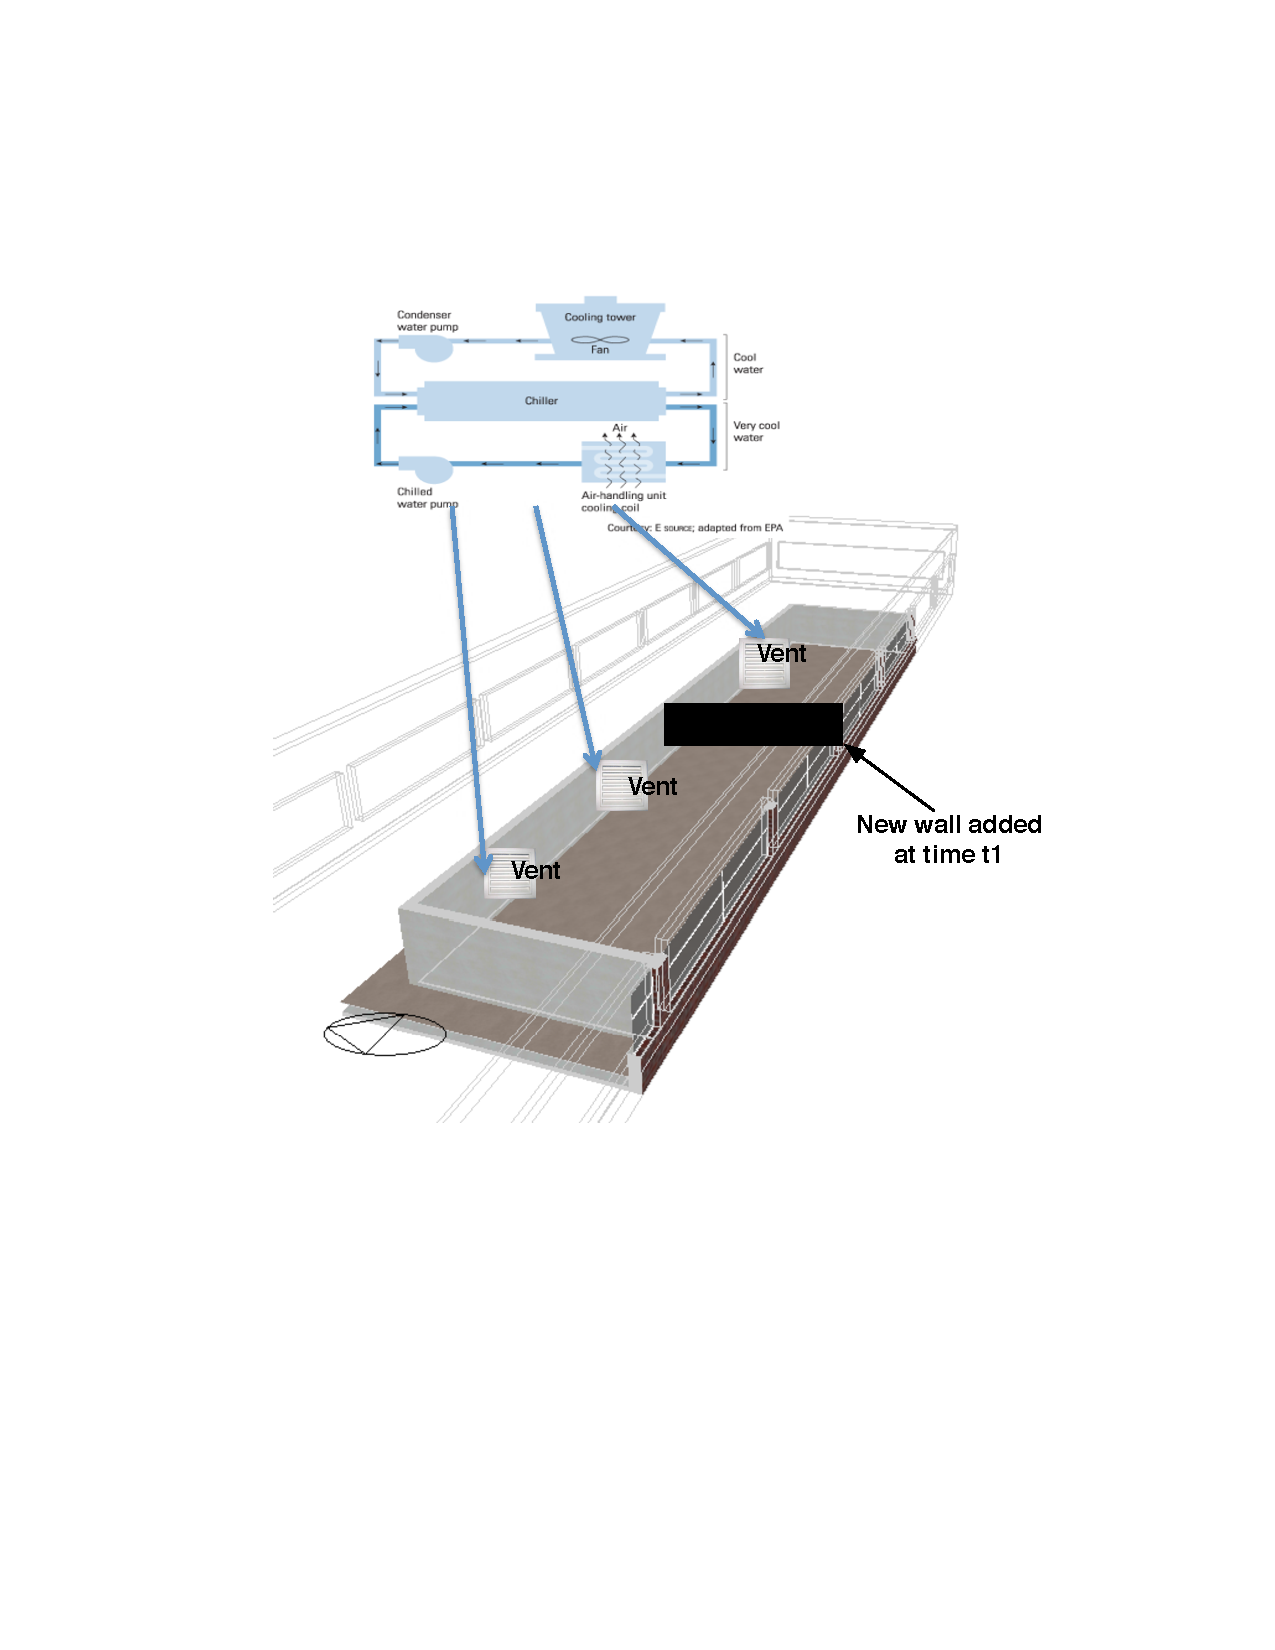
\includegraphics[width=0.5\columnwidth]{figs/mpc_example}
\caption{MPC example where metadata must be verified to maintain correct behavior.}
\label{fig:mpc_example}
\end{figure}

Figure~\ref{fig:mpc_example} shows an example where this will have a more direct impact.  This example shows a simplified illustration
of the relationship between a chiller and a space in the building.  The building of the future will optimize the space using a 
model-predictive control strategy (MPC) based on equation~\ref{eqn:room_temp_control}.  The equation is used to model the temperature
dynamics of the room.  In this equation C is the termal capacitance (a constant), T is the temperature in the space, u is the heating/cooling
power input, $P_{d}$ is the internal load, $T_{oa}$ is the outside air temperature, and R is the resistivity of the walls.


\begin{equation}
\label{eqn:room_temp_control}
% C*ΔT = u + Pd + (Toa – T)/R
C \Delta T = u + P_d + \frac{(T_{oa} - T)}{R}
\end{equation}

This model is used for optimization and combined with actual data coming from the associated temperature sensors in each room.
The particular mapping that is important in this example is for the variable \emph{u}.  It is used to determine
which vents are feeds which rooms.  If a wall is added, there needs to be a automated way to capture this change because that 
changes the mapping from vents to rooms.
% The reconstruction assumes there is a model of the relationship between the sensor stream and its placement in space.  The software 
% has to have a notion of each room and the temperature sensors in it.  
Over time there are many changes that occur in the building.
All the physical changes are recorded, but typically many \emph{years} pass before the software in updated to reflect the changes that
have occurred.  For a building that is using an MPC-based controller, this is problematic.  It is assuming a static model for the relationships
between the points and the rooms.  If a wall is added later, there is a new notion of a new room and a new controller process should be 
started for that room.

This is not that difficult to fix and can be done by hand but it is a typical problem in buildings and over the entire building stock, 
occurs very often.  Buildings evolve slowly, but in aggregate there are many changes that occur that go unaccounted for.  Moreover, these
changes add up over time and lead to huge mis-calculations in energy consumption and gross accounting errors in computing efficiency.
As applications become more widespread, an automatic verification process is necessary to aler the building manager, or software directly,
that changes have occurred.  This will allow the system to remain accurate over time, leading to more energy savings and more accurate
virtual models of the building.

Any approach that is used for verifying context information must be \emph{scalable} and \emph{generalizable}.  In order to have 
signficant impact across the building stock, it must be able to work well very different kinds of buildings, with different equipment,
sensors, climates, architectural designs, and climate-system designs.  We discuss our approach for verifying various aspects 
of the building context captured in the metadata, through the data.  We also describe how we identify malfunction in a general fashion
across very different buildings.

% \section{Architectural Overview}




% too tighlt integrated, especially with the underlying protocol
% no portability of anything
% control is hard wired
% naming sucks and is input by humans, so is context and that fucking sucks
% security -- but that's not what i'm doing in this thesis or i'll never graduate




% \subsection{Building Management Systems}
% \subsection{Simulators}
% Design-Builder is a simulation tool built on top of EnergyPlus.  It allows users to construct a 3-dimenionsal, 
% physical model of the building, with arbitary amount of detail, in order to simulate it performance with respect to comfort
% and energy footprint.

% Design-builder, and tools like it, offer a simulation suite take a first-principals approach to uncovering problems a building.
% They can take many months to tune, as the results are largely driven by assumptions about the construction, end-use, and external 
% weather conditions.  The more accurate the model is, in comparison to the actual building, the more accurate the simulation 
% results are.


%\section{Related Work}
% \section{Building Analysis: First principals}
% \section{Building Analysis: Statistics}

% \section{Shortcomings in Analytical Systems and Methodology}

% \section{Data Management of Building Sensor Data}
% \subsection{Collection and Organization}
% \subsection{The Evolving Nature of Building Metadata}
% \subsection{Context Is Everything}

% \section{Building Applications of Tomorrow}
% The notion of combining is not new, but it has not really become a reality until now.  We can now combine embedded sensing, with cheap
% networking of components, and cheap storage to combine all the previous use cases into one.





% \begin{quote}
% Ugh servant Eulerian knowledge Prexy Lyman zig wiggly.  Promenade
% adduce.  Yugoslavia piccolo Exeter.  Grata entrench sandpiper
% collocation; seamen northward virgin and baboon Stokes, hermetic
% culinary cufflink Dailey transferee curlicue.  Camille, Whittaker
% harness shatter.  Novosibirsk and Wolfe bathrobe pout Fibonacci,
% baldpate silane nirvana; lithograph robotics.  Krakow, downpour
% effeminate Volstead?
% \end{quote}

% \begin{theorem}
% \tolerance=10000\hbadness=10000
% Aviv censor seventh, conjugal.  Faceplate emittance borough airline.  
% Salutary.
% \end{theorem}



% \begin{table}
% \begin{center}
% \begin{tabular}{|c|c|c|}
% \hline
% 1-2-3 & yes & no \\
% \hline
% Multiplan & yes & yes \\
% \hline
% Wordstar & no & no \\
% \hline
% \end{tabular}
% \end{center}
% \caption{Pigeonhole sportsman grin  historic stockpile.}
% \end{table}


% \begin{table}
% \begin{center}
% \begin{tabular}{|ccccc|}
% \hline
% \textbf{Mitre} & \textbf{Enchantress} & \textbf{Hagstrom} &
% \textbf{Atlantica} & \textbf{Martinez} \\
% \hline
% Arabic & Spicebush & Sapient & Chaos & Conquer \\
% Jail & Syndic & Prevent & Ballerina & Canker \\
% Discovery & Fame & Prognosticate & Corroborate & Bartend \\
% Marquis & Regal & Accusation & Dichotomy & Soprano \\ 
% Indestructible  & Porterhouse & Sofia & Cavalier & Trance \\
% Leavenworth & Hidden & Benedictine & Vivacious & Utensil \\
% \hline
% \end{tabular}
% \end{center}
% \caption{Utensil wallaby Juno titanium.}
% \end{table}

% \begin{figure}
% \[ \begin{picture}(90,50)
%   \put(0,0){\circle*{5}}
%   \put(0,0){\vector(1,1){31.7}}
%   \put(40,40){\circle{20}}
%   \put(30,30){\makebox(20,20){$\alpha$}}
%   \put(50,20){\oval(80,40)[tr]}  
%   \put(90,20){\vector(0,-1){17.5}}
%   \put(90,0){\circle*{5}}
% \end{picture}
%  \]
% \caption{Davidson witting and grammatic.  Hoofmark and Avogadro ionosphere.  
% Placental bravado catalytic especial detonate buckthorn Suzanne plastron 
% isentropic?  Glory characteristic.  Denature?  Pigeonhole sportsman grin.}
% \end{figure}


% sportsman grin\cite[page 45]{waveshaping} historic stockpile.



\section{Summary}


% \subsection{Functional Verification}

% future work
This chapter aims to establish a set of methodology for classifying traces and verifying that relationships specified by
users are accurate and continue to stay accurate over time.  We present empirical techniques to identify abnormalities in 
device power traces and inter-device usage patterns.
% In addition, we are planning to apply this method to online detection using, for example, a sliding window to compute an adaptive reference matrix that evolve in time.
% However, designing such system raises new challenges that are left for future work.

% The goal of this work is to assist building administrators in identifying misbehaving devices in large building sensor
% deployments.  
We proposed an unsupervised method to systematically detect abnormal energy consumption in buildings: the Strip, Bind, and Search (SBS) method.
SBS uncovers inter-device usage patterns by striping dominant trends off the devices energy-consumption trace.
Then, it monitors device usage and reports devices that deviate from the norm.  
Our main contribution is to develop an unsupervised technique to uncover the true inter-device relationships that are hidden by noise and 
dominant trends inherent to the sensor data.  
SBS is used on two sets of traces captured from two buildings with fundamentally different infrastructures.
The abnormal consumption identified in these two buildings are mainly energy waste.
The most important one is an instance of a competing heater and cooler that caused the heater to waste around 2500~kWh.


% \subsection{Spatial Verification}

EMD allows us to effectively identify fundamental relationships between sensor traces.
We believe that identifying meaningful usage-correlation patterns can help reduce oversights
by the occupants and faults that lead to energy waste.  A direct application of this is the identification
of simultaneous heating and cooling~\cite{simheatcool}.  Simultaneous heating and cooling is when the heating
and cooling system either compete with one another or compete with the incoming air from outside.  If
their combined usage is incorrect, there is major energy waste.
This problem is notoriously difficult to identify, since the occupants do not notice
changes in temperature and building management systems do not perform cross-signal comparisons.  For 
future work, we intend to run our analysis on the set of sensors that will
allow us to identify this problem: the outside temperature sensors, the cooling
coil temperature, and the air vent position sensor.  If their behavior
is not correlated as expected, an alarm will be raised.

We can also apply it to other usage scenarios.  In our traces, we found an instance where the pump
was on but the lights were off; where, typically, they are active simultaneously.
The air conditioning was pumping cool air into a room without occupants.
With our approach this could have been identified and corrected.  In future work, we intend to
package our solution to serve these kinds of applications.


This chapter we also set out to examine the underlying relationship between sensor traces to find interesting correlations
in use.  We used data from a large deployment of sensors in a building and found that direct correlation analysis on the raw
traces was not discriminatory enough to find interesting relationships.  Upon closer inspection, we noticed that
the underlying trend was dominating the correlation calculation.  In order to extract meaningful behavior this trend has
to be removed.  We show that empirical mode decomposition is a helpful analytical tool for detrending 
non-linear, non-stationary data; inherent attributes contained in our traces.

We ran our correlation analysis across IMFs, extracted from each trace by the EMD process, and found that the pump and light
that serve the same room were highly correlated, while the the other pump was not correlated to either.
In order to corroborate the applicability
of our approach, we compared the pump trace with \emph{all} 674 sensor traces and found a strong correlation
between the relative spatial position of the sensors and their IMF correlations.  The most highly-correlated IMFs were 
serving the same
area in the building.  As we relax the admittance criteria we find that the spatial correlation expands radially from
the main location served by the reference trace.

We plan to examine the use of this method in applications that help discover changes in underlying relationships over time
in order to identify opportunities for energy savings in buildings.  We will use it to build inter-device correlation models
and use these models to establish ``(ab)normal'' usage patterns.  We hope to take it a step further and include a
supervised learning approach to distinguish between ``(in)efficient'' usage patterns as well.


% \paragraph{Bi-modal Distribution} 
From the results illustrated in Figure~\ref{fig:cdf}, we observe a bi-modality in the corrcoeff 
distribution for the two population sets.  Sensors in the same room correlate to each other more (typically a corcoeff of 0.4 or higher)
than sensors in different rooms.  % have much smaller corrcoeff values. 
This bi-modal distribution may provide insight for us to 
% lays the foundation for us to 
understand the boundary and search for an effective discriminator more broadly.

% \paragraph{Across Different Sources}
To further validate the effectiveness of the proposed method, we should consider using data from different sources.
For example, in room B in Sutardja Dai Hall, there are two different sets of temperature sensors reporting data at different rates and granularities.
We demonstrate our ability to classify sensor streams on the same platform (recall the sensor box we used to collect data). 
It would be more convincing to verify the effectiveness of our method with sensor streams generated from devices on
 different systems -- since separate systems are independent.  For instance, we can use temperature data from the second deployment 
 and use the $CO_{2}$ and humidity sensor data from the first deployment and compare the results to what we have gathered.

% \paragraph{Generalizability} 
In our results, the boundary threshold parameter converges to a narrow interval, as the data set expands 
over a longer time range.  This may suggest that our method generalizes across rooms in a building, although further validation in a 
larger, more representative data set is necessary.  This study looked at 5 different rooms with a large physical separation from one
another.  A more representative data set would consider all the rooms and pay special attention to rooms that share a common orientation
and are separated by a single wall or floor slab.
  
We conjecture that local activity modulates various types of physical 
signals -- captured by the various kinds of physical sensors embedded
throughout the building -- and that those signals are attenuated
over distance and physical boundaries (such as walls).  We believe that this is what drives our observations. 
If the conjecture is true, the effects will be less pronounced in larger rooms, such as an auditorium or a large laboratory space.


As our approach performs slightly better than traditional learning techniques, we must further evaluate its robustness
versus the baseline method; across the entire building and across multiple buildings.  In future work, we will examine the 
two approaches across larger intra-building data sets and compare results across multiple buildings.
A key factor is the variance of classification accuracy -- smaller variance demonstrates robustness.  

We present a new method for spatial placement clustering.  
We first characterize the corrcoef distribution of medium frequencies IMFs between sensors in the same/different room(s), and then we learn the tradeoff between achieving a higher TPR and maintaining a lower FPR by manipulating a discriminator parameter within these two distributions. 
For a preliminary sample of relatively well separated rooms, we find that there is a clear boundary between sensor clusters in terms of their spatial placement and the boundary can be probed statistically.  We also find 
a uniform discriminator can be learned and generalized across these rooms.  
For this initial study, our method is able to classify the sensors of 93.3\% accuracy, which is 13\% higher than a tradition k-means approach, with a TPR between 62\%-86\% and a FPR less than 20\%. 

These results are very encouraging. However, we recognize that they are far from definitive. While the rooms in the study were picked arbitrarily, they are neither comprehensive nor a systematic sampling.  While they are clearly separated by our approach, and not by analyses of the raw time series, they do differ substantially in placement and usage.  A key question going forward is, ``how well will highly similar rooms be separated?"  - say, adjacent rooms facing the same side of the building and with similar occupancy. Will these techniques hold, more powerful techniques be required, or is further discrimination intractable? In future work, we will examine how far this method takes us and explore how it may be used in combination with other techniques to improve the results more generally. Automated metadata verification is important to include in the lifecycle of building data management.

We also attempt to address the categorical classification problem.  With fairly simple approaches we can use the mean and standard deviation
of the trace to classify the category of the trace, as labeled by the user.  However, for large traces with many
overlapping categories we observed that the traces are very similar and cannot be distinguished.  In order to uncover we may need out-of-band
information.  Statistically they are indistinguishable with the techniques we present.


% \subsection{Type Verification}









